\documentclass[a4paper, 12pt]{article}
\usepackage[utf8]{inputenc}
\usepackage[T1]{fontenc}
\usepackage[magyar]{babel}
\usepackage{graphicx}
\usepackage[margin=65 pt]{geometry}
\usepackage{amsmath}
\usepackage{wrapfig}


\begin{document}

\begin{titlepage}\centering
\vspace*{250 pt}
\Huge \textbf{Folytonos közegek mechanikája}

\LARGE \textbf{2. tétel}

\LARGE A deformációs tenzor bevezetése


~

\LARGE Kidolgozta: Pollák Edina

\vspace*{\fill}
\end{titlepage}

\newpage
\part*{\Large{A deformációs tenzor}}

\vspace{30 pt}

Külső erők hatására a test alakváltozáson megy keresztül, ebben a tételben a bonyolultabb deformációkat szeretnénk leírni. Referenciaként azt az állapotot vesszük, amikor a test atomjai egyensúlyban vannak.

~

\begin{figure}[h]
\centering
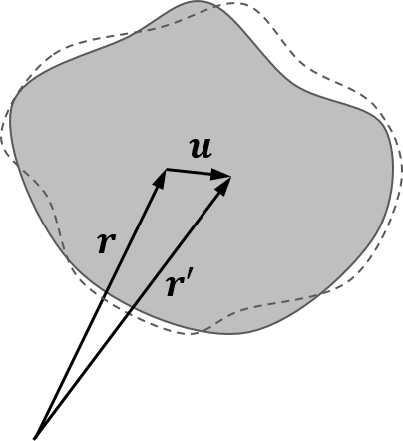
\includegraphics[scale=0.4]{tetel2_1.png}
\caption{}
\end{figure}

Vegyünk egy testet, melynek atomjait $\mathbf{r}$ helyvektorral jellemezhetjük. Deformáció hatására az atom elmozdul, módosult helyzetét egy $\mathbf{r'}$ helyvektor írja majd le. Bevezetjük az $\mathbf{u(r)}=\mathbf{r'}-\mathbf{r}$ vektormezőt a deformáció jellemzésére (1. ábra).

Az alakváltozás során kialakuló belső erők nem függhetnek direkten $\mathbf{u}$-tól, mert egyszerű eltolásra, $\mathbf{u}=\mathrm{konstans}$ esetén nincsenek belső erők (ld. merev testek).

~

Vizsgáljuk a relatív megnyúlást.

\begin{figure}[h]
\centering
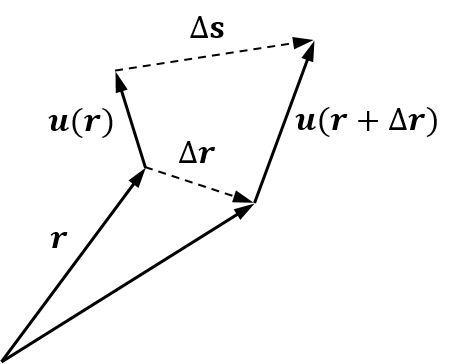
\includegraphics[scale=0.4]{tetel2_2.png}
\caption{}
\end{figure}

Ehhez az $\mathbf{r}$ és $\mathbf{r}+\Delta\mathbf{r}$ helyvektorral jellemzett részecskék útját követjük. Az eredeti távolság ($\Delta\mathbf{r}$) és a megváltozott távolság ($\Delta\mathbf{s}$) vektorai közötti kapcsolat (a 2. ábra alapján):

$$\Delta\mathbf{s}=\mathbf{r}+\Delta\mathbf{r}+\mathbf{u}(\mathbf{r}+\Delta\mathbf{r})-\mathbf{r}-\mathbf{u}(\mathbf{r})$$

$$\Delta\mathbf{s}=\Delta\mathbf{r}+\mathbf{u}(\mathbf{r}+\Delta\mathbf{r})-\mathbf{u}(\mathbf{r})$$

A gradiens definíciója szerint:

$$\Phi(\mathbf{r}+\Delta\mathbf{r})-\Phi(\mathbf{r})\approx \mathrm{grad}\Phi\cdot\Delta\mathbf{r}$$

$$u_j(\mathbf{r}+\Delta\mathbf{r})-u_j(\mathbf{r})\approx \frac{\partial u_j}{\partial r_i}\cdot\Delta r_i$$

Ennek mintájára vektormező esetén komponensenként értelmezünk egy gradienst, ami egy kétindexes tenzor lesz. Jelen eseteben az $\mathbf{u}(\mathbf{r})$ vektormezőhöz tartozó gradienst disztorziónak nevezzük:

$$\Delta u_j=\beta_{ij}\Delta r_i$$

$$\Delta \mathbf{u}=\mathbf{\hat\beta^{T}}\Delta r_i$$

Ezek alapján

$$|\Delta\mathbf{s}|=\sqrt{(\Delta r_i+\beta_{ji}\Delta r_j)(\Delta r_i+\beta_{ki}\Delta r_k)}$$

alakban kifejezhető a $\Delta\mathbf{s}$ vektor hossza (önmagával vett skaláris szorzata), és felírható a

$$\frac{\Delta|\Delta\mathbf{s}|}{|\Delta\mathbf{r}|}=\frac{\sqrt{(\Delta r_i+\beta_{ji}\Delta r_j)(\Delta r_i+\beta_{ki}\Delta r_k)}}{|\Delta\mathbf{r}|}-\frac{|\Delta\mathbf{r}|}{|\Delta\mathbf{r}|}$$

relatív megnyúlás. 

~

A zárójeleket kibontva:

$$\frac{\Delta|\Delta\mathbf{s}|}{|\Delta\mathbf{r}|}=\frac{\sqrt{|\Delta\mathbf{r}|^2+\Delta r_i\beta_{ji}\Delta r_j+\Delta r_i\beta_{ki}\Delta r_k+\Delta r_j\beta_{ji}\beta{ki}\Delta r_k}}{|\Delta\mathbf{r}|}-1$$

A $\beta^2$-et tartalmazó tagok elhanyagolhatóan kicsik, mert kicsit a deformáció:

$$\frac{\Delta|\Delta\mathbf{s}|}{|\Delta\mathbf{r}|}=\frac{\sqrt{|\Delta\mathbf{r}|^2+\Delta r_i\beta_{ji}\Delta r_j+\Delta r_i\beta_{ki}\Delta r_k}}{|\Delta\mathbf{r}|}-1$$

A $\Delta r_i\beta_{ji}\Delta r_j$ kifejezés $i,j$-ben szimmetrikus, a $\beta$ tenzor pedig felbontható egy szimmetrikus és egy antiszimmetrikus részre. Szimmetrikus és antiszimmetrikus kifejezések szorzata $0$-t ad (indexcserékkel belátható). Tehát $\beta$ antiszimmetrikus részére a kifejezés $0$, így az egyenlő a $\beta$ szimmetrikus részét - ami a továbbiakban legyen $\varepsilon$ deformációs tenzor - tartalmazó kifejezéssel,: $\Delta r_i\beta_{ji}\Delta r_j=\Delta r_i\varepsilon_{ji}\Delta r_j$. 

~

A deformációs tenzor pontosabb meghatározása:

$$\varepsilon_{ij}=\frac12(\beta_{ij}+\beta{ji})=\frac12\left(\frac{\partial u_i}{\partial r_j}+\frac{\partial u_j}{\partial r_i}\right)$$

Vezessük be a $\frac{\Delta\mathbf{r}}{|\Delta\mathbf{r}|}=\mathbf{n}$ vektort, ezáltal a relatív megnyúlás a következp alakra hozható:

$$\frac{\Delta|\Delta\mathbf{s}|}{|\Delta\mathbf{r}|}=\sqrt{1+2\cdot n_i\varepsilon_{ij}n_j}-1$$

Taylor-soros közelítést alkalmazva:

$$\frac{\Delta|\Delta\mathbf{s}|}{|\Delta\mathbf{r}|}\approx 1+\frac12\cdot 2\cdot n_i\varepsilon_{ij}n_j-1=n_i\varepsilon_{ij}n_j=\mathbf{n}\mathbf{\hat\varepsilon}\mathbf{n}$$

Ez megadja a helyfüggő epszilon ismeretében a test egy adott pontjában az $\mathbf{n}$ irányú relatív megnyúlást.


\part*{\Large{A relatív térfogatváltozás}}

\begin{figure}[h]
\centering
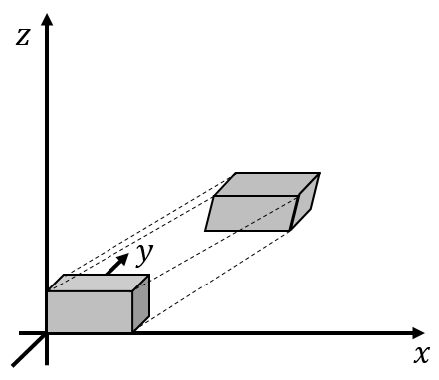
\includegraphics[scale=0.6]{tetel2_3.png}
\caption{}
\end{figure}

Veszünk egy apró téglatestet (3. ábra), melynek élein futó vektorok az alábbiak:

$$\Delta\mathbf{x}= \left( \begin{array}{c} \Delta x\\0\\0\end{array}\right)$$

$$\Delta\mathbf{y}= \left( \begin{array}{c} 0\\ \Delta y\\0\end{array}\right)$$

$$\Delta\mathbf{z}= \left( \begin{array}{c} 0\\0\\\Delta z\end{array}\right)$$

Ha a téglatest deformációt szenved, az élvektorok így fognak változni a korábbiak alapján:

$$\Delta\mathbf{r'}=\Delta\mathbf{r}+\Delta \mathbf{r} \beta$$

$$\Delta r'_i=\Delta r_i+\beta_{ji}\Delta r_j=(\delta_{ij}+\beta_{ji})\cdot \Delta r_j$$

Egyenként kiírva:

$$\Delta\mathbf{x'}= \left( \begin{array}{c} 1+\beta_{11}\\\beta_{12}\\ \beta_{13}\end{array}\right)\Delta x$$

$$\Delta\mathbf{y'}= \left( \begin{array}{c} \beta_{21}\\1+\beta_{22}\\ \beta_{23}\end{array}\right)\Delta y$$

$$\Delta\mathbf{z'}= \left( \begin{array}{c} \beta_{31}\\\beta_{32}\\ 1+\beta_{33}\end{array}\right)\Delta z$$

Vegyesszorzatuk megadja a deformált téglalap - paralelepipedon - térfogatát, ami átírható a mátrixba rendezett vektorok determinánsaként. 

Ebből felírható a kezdeti ($V=\Delta x\Delta y\Delta z$) és végső térfogatok aránya:

 $$\frac{\Delta V'}{V}=\begin{vmatrix}
1+\beta_{11} & \beta_{12} & \beta_{13} \\ 
\beta_{21} & 1+\beta_{22} & \beta_{23}\\ 
\beta_{31} & \beta_{32} & 1+\beta_{33} 
\end{vmatrix}$$

Ezt kibontva, és $\mathbf{\hat\beta}$-ban 1-nél és magasabb rendű tagokat elhanyagolva (mivel a kísérleti tapasztalat szerint a deformáció kicsi):

$$\frac{\Delta V'}{V}=1+\beta_{11}+\beta_{22}+\beta_{33}$$

Ebből megkaphatjuk a relatív térfogatválzoást:

$$\frac{\Delta V}{V}=\frac{V'-V}{V}=\mathrm{Sp} \mathbf{\hat\beta}$$

Mivel $\mathbf{\hat\beta}$ antiszimmetrkus részénk diagonálelemei 0-k: $\mathrm{Sp} \mathbf{\hat\beta}=\mathrm{Sp} \mathbf{\hat\varepsilon}$, tehát:

$$\frac{\Delta V}{V}=\mathrm{Sp} \mathbf{\hat\varepsilon}$$

Ez tehát a relatív térfogatváltozás a deformációs tenzor segítségével kifejezve.

Epszilon definícióját felhasználva ez tovább alakítható:

$$\frac{\Delta V}{V}=\frac{\partial u}{\partial x}+\frac{\partial u}{\partial y}+\frac{\partial u}{\partial z}=\mathrm{div}~\mathbf{u}$$

Látható, hogy a deformáció csak $\mathbf{\hat\varepsilon}$ tenzor diagonális elemeitől függ. A nem diagonális elemek ezek szerint a tiszta nyíráshoz tartoznak.



\end{document}